\documentclass{article}% [Determines font size] { }Determines type of document (article/beamer/book/etc.)

\usepackage{subcaption}% Required package for subfigure environment.
\usepackage{graphicx}% Required package to compile figures.
\usepackage{blindtext}

\begin{document}% Required to produce a compiled LaTeX document. 

\blindtext

\begin{figure}[h]% 
        \caption{Multiple figures}% Caption for the whole figure, placed at the top before the subfigure environment. 
    \begin{subfigure}{0.5\textwidth}% Create a subfigure environment environment for each figure that are being grouped together. Second command defines the size of subfigure environment.
            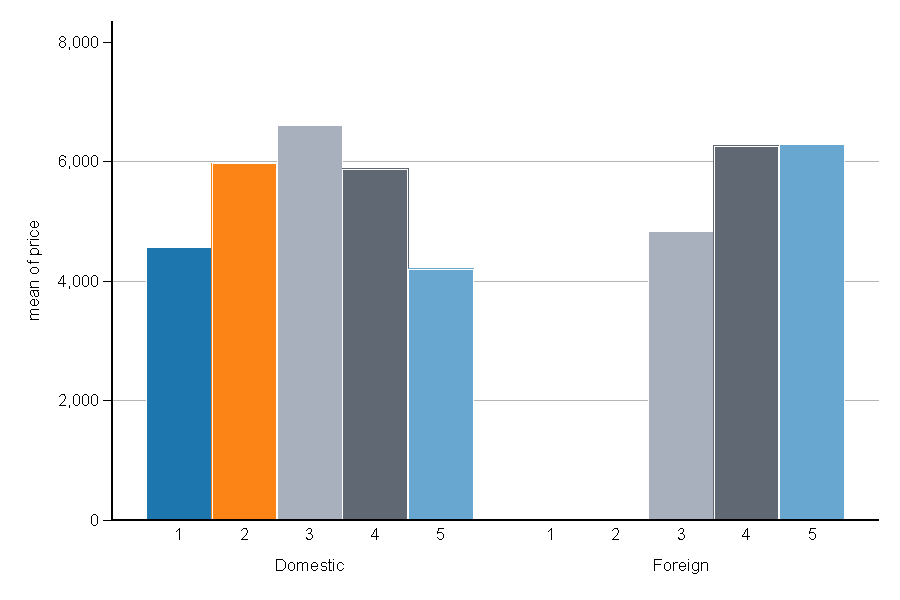
\includegraphics[width=1\linewidth]{figure1.pdf}% Width is based on the space of the subfigure environment. Therefore 100% width is just 50% of total textwidth.
            \caption{First figure}% Subfigure caption, placed below subfigure.
            \label{fig:subfigure_a}%Use a ":" to create a category of labels on the left side, and the right side is the label of this specific figure.
    \end{subfigure}
    \begin{subfigure}{0.5\textwidth}% Make sure there is no space between end and begin subfigure commands to make subfigures places side-by-side.
            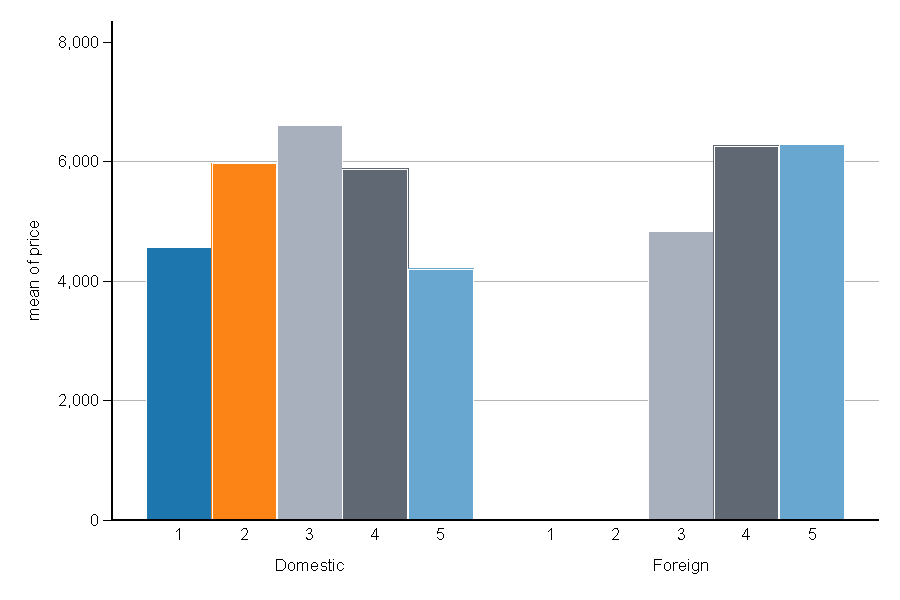
\includegraphics[width=.75\linewidth]{figure1.pdf}% 
            \caption{Second figure}% 
            \label{fig:subfigure_b}%
    \end{subfigure}
\end{figure}

\blindtext[4]


\end{document}